% \documentclass[handout]{beamer}
\documentclass{beamer}

\mode<presentation>
{
  \usetheme{default}
  % \usefonttheme[onlymath]{serif}
  % \usetheme{Singapore}
  % \usetheme{Warsaw}
  % \usetheme{Malmoe}
  % \useinnertheme{circles}
  % \useoutertheme{infolines}
  % \useinnertheme{rounded}

  \setbeamercovered{transparent=20}
}

\usepackage[english]{babel}
\usepackage[latin1]{inputenc}
\usepackage{alltt,listings,multirow,ulem,siunitx}
\usepackage[absolute,overlay]{textpos}
\TPGrid{1}{1}
\usepackage{pdfpages}
\usepackage{ulem}
\usepackage{multimedia}
\usepackage{multicol}
\usepackage{transparent}
\newcommand\hmmax{0}
\newcommand\bmmax{0}
\usepackage{bm}
\usepackage{comment}
\usepackage{subcaption}

% font definitions, try \usepackage{ae} instead of the following
% three lines if you don't like this look
\usepackage{mathptmx}
\usepackage[scaled=.90]{helvet}
% \usepackage{courier}
\usepackage[T1]{fontenc}
\usepackage{tikz}
\usetikzlibrary{decorations.pathreplacing}
\usetikzlibrary{shadows,arrows,shapes.misc,shapes.arrows,shapes.multipart,arrows,decorations.pathmorphing,backgrounds,positioning,fit,petri,calc,shadows,chains,matrix,mindmap}

\newcommand\vvec{\bm v}
\newcommand\bvec{\bm b}
\newcommand\bxk{\bvec_0 \times \kappa_0 \cdot \nabla}
\newcommand\delp{\nabla_\perp}

% \usepackage{pgfpages}
% \pgfpagesuselayout{4 on 1}[a4paper,landscape,border shrink=5mm]

\usepackage{JedMacros}

\newcommand{\timeR}{t_{\mathrm{R}}}
\newcommand{\timeW}{t_{\mathrm{W}}}
\newcommand{\mglevel}{\ensuremath{\ell}}
\newcommand{\mglevelcp}{\ensuremath{\mglevel_{\mathrm{cp}}}}
\newcommand{\mglevelcoarse}{\ensuremath{\mglevel_{\mathrm{coarse}}}}
\newcommand{\mglevelfine}{\ensuremath{\mglevel_{\mathrm{fine}}}}

%solution and residual
\newcommand{\vx}{\ensuremath{x}}
\newcommand{\vc}{\ensuremath{\hat{x}}}
\newcommand{\vr}{\ensuremath{r}}
\newcommand{\vb}{\ensuremath{b}}

%operators
\newcommand{\vA}{\ensuremath{A}}
\newcommand{\vP}{\ensuremath{I_H^h}}
\newcommand{\vS}{\ensuremath{S}}
\newcommand{\vR}{\ensuremath{I_h^H}}
\newcommand{\vI}{\ensuremath{\hat I_h^H}}
\newcommand{\vV}{\ensuremath{\mathbf{V}}}
\newcommand{\vF}{\ensuremath{F}}
\newcommand{\vtau}{\ensuremath{\mathbf{\tau}}}


\title{Computational Science and Engineering}
\author{Jed Brown}

% - Use the \inst command only if there are several affiliations.
% - Keep it simple, no one is interested in your street address.
% \institute
% {
%   Mathematics and Computer Science Division \\ Argonne National Laboratory
% }

\date{CS Research Retreat, 2017-09-22}
%    - **SW**: miniapps: Nekbone, Laghos, NekCEM Ceedling, HPGMG-FE, HOLMES; CEED distribution/Spack; HO visualization ALPINE, VTK-m, iLight… HO data format; GSLIB; MPICH collaboration; high-order meshes, PUMI; solvers: Strumpack, PETSC, matrix-free; zfp;  

% This is only inserted into the PDF information catalog. Can be left
% out.
\subject{Talks}


% If you have a file called "university-logo-filename.xxx", where xxx
% is a graphic format that can be processed by latex or pdflatex,
% resp., then you can add a logo as follows:

% \pgfdeclareimage[height=0.5cm]{university-logo}{university-logo-filename}
% \logo{\pgfuseimage{university-logo}}



% Delete this, if you do not want the table of contents to pop up at
% the beginning of each subsection:
% \AtBeginSubsection[]
% {
% \begin{frame}<beamer>
%   \frametitle{Outline}
%   \tableofcontents[currentsection,currentsubsection]
% \end{frame}
% }

\AtBeginSection[]
{
  \begin{frame}<beamer>
    \frametitle{Outline}
    \tableofcontents[currentsection]
  \end{frame}
}

% If you wish to uncover everything in a step-wise fashion, uncomment
% the following command:

% \beamerdefaultoverlayspecification{<+->}

\begin{document}
\lstset{language=C}
\normalem
\setbeamercolor{background canvas}{bg=}
\setbeamertemplate{navigation symbols}{}

\begin{frame}
  \begin{center}
    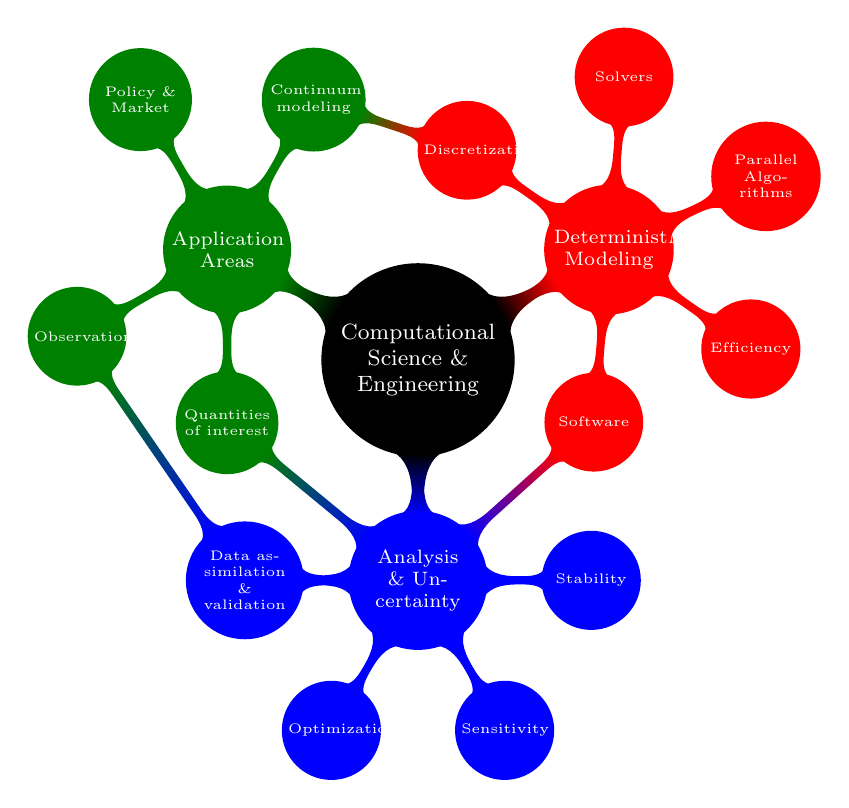
\begin{tikzpicture}
      [small mindmap,concept color=black,text=white,
      %level 1 concept/.append style={level distance=120,sibling angle=30},
      extra concept/.append style={color=blue!50,text=black}]

      \node [concept] {Computational Science \& Engineering}
      child [concept color=green!50!black,grow=150] {
        node [concept] {Application \\ Areas}[counterclockwise from=60]
        child {node [concept] (cont) {Continuum modeling}}
        child {node [concept] (policy) {Policy \& Market}}
        child[grow=-150] {node [concept] (obs) {Observation}}
        child[grow=-90] {node [concept] (qoi) {Quantities of interest}}
      }
      child [concept color=red,text=white,grow=30] {
        node [concept] {Deterministic Modeling}[clockwise from=145,sibling angle=25]
        child {node [concept] (disc) {Discretization}}
        child {node [concept] (solver) {Solvers}}
        child {node [concept] (alg) {Parallel Algorithms}}
        child {node [concept] (eff) {Efficiency}}
        child {node [concept] (software) {Software}}
      }
      child [concept color=blue,text=white,grow=-90] {
        node[concept] (analysis) {Analysis \& Uncertainty}[clockwise from=0]
        child {node [concept] (stab) {Stability}}
        child {node [concept] (sens) {Sensitivity}}
        child {node [concept] (opt) {Optimization}}
        child {node [concept] (assim) {Data assimilation \\ \& validation}}
      }
      ;
      \begin{pgfonlayer}{background}
        \path (analysis) to[circle connection bar switch color=from (blue) to (red)] (software);
        \path (cont) to[circle connection bar switch color=from (green!50!black) to (red)] (disc);
        \path (qoi) to[circle connection bar switch color=from (green!50!black) to (blue)] (analysis);
        \path (obs) to[circle connection bar switch color=from (green!50!black) to (blue)] (assim);
      \end{pgfonlayer}
    \end{tikzpicture}
  \end{center}
\end{frame}


\begin{frame}{Physics-based models, data science, and machine learning}
  \begin{itemize}
  \item Direct observation often impossible/prohibitively expensive
  \item Sparse, indirect measurements
  \item Conservation: mass, momentum, energy, entropy inequality
  \item Engineering reliability
  \item Hazard assessment, rare events
  \item Design optimization, especially with gradients
  \end{itemize}
\end{frame}

% \includepdf[pages=16]{/home/jed/na-slides/Keyes-ExaflopsSeriously-2011}

\begin{frame}{Parallel scientific computing for scientists and engineers}
  \begin{itemize}
  \item[CEAE] Richard Regueiro, Hari Rajaram, Scott Runnels (LANL)
  \item[Aero] Kurt Maute, John Evans, Ken Jansen
  \item[CS/RC] Thomas Hauser
  \item Development of parallel software
  \item Discretization of partial differential equations
  \item Parallel algebraic solvers, PETSc
  \end{itemize}
\end{frame}

\begin{frame}{Curriculum coordination}
  \begin{itemize}
  \item Undergrad level, across the college
    \begin{itemize}
    \item Probability and statistics
    \item Simple physically based models
    \item ``black-box'' regression, etc.
    \item Intro to dynamical systems
    \end{itemize}
  \item Advanced undergrad and grad level
    \begin{itemize}
    \item Numerical methods for partial differential equations
    \item Numerical optimization
    \item Data assimilation in high dimensions
    \item Uncertainty quantification, beyond Gaussian
    \item Fast algorithms (multigrid, fast multipole, compressive sensing)
    \item Efficient, maintainable, extensible parallel computing
    \end{itemize}
  \item Our ``CS\&E'' faculty: Xiao-Chuan Cai, Liz Jessup, Henry Tufo, Jed Brown, Abtin Rahimian, Paul Constantine, Didem Unat*, Rebecca Morrison*, David Hall
  \item Many others use these tools
  \end{itemize}
\end{frame}

\end{document}
